\section{Introduction}
\label{sec:intro}

% Role: opening. Message: self-improvement methods vary beyond their model calls.
Agent self-improvement changes the system around a model as well as the instructions sent to it. GEPA searches prompt components using reflective feedback~\citep{agrawal2026gepareflectivepromptevolution,gepa_code}; ACE accumulates a structured playbook~\citep{zhang2026agenticcontextengineeringevolving,ace_code}; Meta-Harness searches executable memory and orchestration code~\citep{lee2026metaharnessendtoendoptimizationmodel,meta_harness_code}; Combee reorganizes prompt learning through parallel aggregation~\citep{li2026combeescalingpromptlearning,gepa_code}; and CORAL coordinates persistent discovery agents~\citep{qu2026coralautonomousmultiagentevolution,coral_code}. These approaches expose different experimental objects, update schedules, and forms of evidence. Studying them in a common system therefore requires preserving their algorithmic distinctions while making their execution and records compatible.

\begin{figure}[t]
\centering
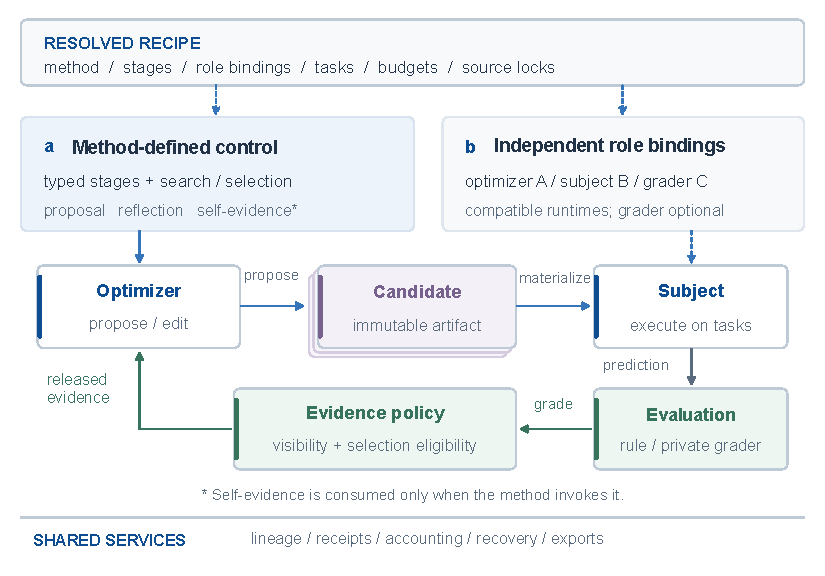
\includegraphics[width=\linewidth]{figures/architecture.pdf}
\caption{\textbf{A common experimental substrate, with method-specific control.} A resolved recipe binds method-defined control and independent harness roles. The central path separates proposal, immutable candidate materialization, and task execution. Formal evaluation returns evidence only through the declared visibility and selection policy. Typed stages, including optional self-evidence, are invoked by the method; the depicted services do not prescribe one universal optimization loop. The lower band preserves common execution records.}
\label{fig:architecture}
\end{figure}

% Role: challenge. Message: the experimental unit includes roles and evidence.
A reproducible self-improvement experiment is larger than an optimizer function. The researcher must identify the exact candidate that ran, the harness and model that proposed it, the subject that executed it, and the evaluator that assigned its score. An interrupted call may have incurred cost without returning a usable result. A hidden test may be recorded for the owner but must remain unavailable to the next proposal. A source edit may exist on disk without ever becoming the executing agent. If these distinctions are implicit, an apparent improvement can instead reflect a changed runtime, leaked feedback, a different selection rule, or missing work.

% Role: method. Message: Proteus separates algorithm from execution contracts.
\proteus{} makes these experimental choices separate, versioned contracts. A \emph{method} owns the optimization loop; \emph{stages} implement typed transformations; \emph{candidates} identify immutable artifacts; and \emph{harness roles} bind model-backed work to execution adapters. Subjects run candidates on tasks, while evaluators produce formal measurements and control their disclosure. Search policies, parallel workflows, persistent workers, accounting, and recovery are shared services rather than mandatory steps in one universal algorithm. Figure~\ref{fig:architecture} summarizes the boundaries.

% Role: advantage. Message: harness agnosticism is bounded role independence.
Harness agnosticism means that a method does not select an adapter through a hard-coded method--harness pair. A recipe can bind a coding proposer and a task subject to the same integration or to different compatible integrations, and can choose their models separately. This is an interface property with concrete limits: a playbook, a prompt overlay, and a source tree still need the correct subject protocol. A supported adapter name does not make every method, role, session mode, or artifact combination valid. Preflight checks and an explicit evidence matrix define the supported subset.

% Role: contribution. Message: the contribution is reusable infrastructure.
The report makes three contributions. First, it specifies a common decomposition of method, typed stage, artifact, harness role, and evaluator, with concrete ACE--Combee and GEPA--Combee compositions. Second, it presents Native as a reference self-evolution method: goals and external scores remain separate, the harness can revise its own tests, and the common profile advances viable candidates without an outer score filter while preserving completed but nonviable candidate edits for repair. Third, it presents a traceable inventory separating historical adapted studies, bounded live role pilots, and source-bound engineering qualification. Existing evolution toolkits already provide extensible infrastructure; the contribution here is the implemented framework and specified Native protocol, not priority for a unified RSI system or a proven quality advantage. Figure~\ref{fig:native} details the Native state transition.

% Role: evidence and boundary. Message: evidence supports an experimental toolkit.
The evidence supports a research toolkit whose available recipes and failure boundaries can be inspected. Historical AIME and Formula runs contain complete declared task splits, while later pilots exercise specific Pi, DSH, and Codex roles. Current preparation checks cover installed extensions, common-trace composition, candidate activation, and a directed CORAL recovery protocol. Their sources and experimental meanings differ, so we do not pool them into a single benchmark or release gate. Generic builders continue to require new model-result qualification. The intended use is to run, inspect, and extend explicitly specified experiments, with missing evidence remaining visible.
